\subsubsubsubsection{Crossing}
\begin{figure}[h]
\centering
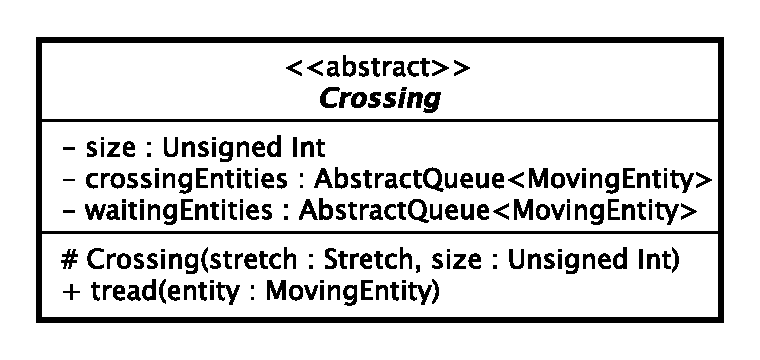
\includegraphics[scale=0.6,keepaspectratio]{images/solution/app/backend/crossing.eps}
\caption{\pReactiveComponentStretchDecoration::Crossing}
\label{fig:sd-app-crossing}
\end{figure}
\FloatBarrier
\begin{itemize}
  \item \textbf{\descr} \\
    It represents the zebra crossing entity. 
  \item \textbf{\attrs}
  \begin{itemize}
    \item \texttt{size: Unsigned Int} \\
The size of the stretch/\texttt{crossingEntities} queue.
    \item \texttt{crossingEntities: AbstractQueue<MovingEntity>} \\
The queue of entities which are granted to cross the zebra crossing stretch.
  \item \texttt{waitingEntities: AbstractQueue<MovingEntity>} \\
The queue of entities which are currently waiting to cross the zebra crossing stretch.
  \end{itemize}
\item \textbf{\ops}
  \begin{itemize}
    \item[\#] \texttt{Crossing(stretch: Stretch, size: Unsigned Int)} \\
Creates a crossing with a specific component and two queues. The
\texttt{crossingEntities} queue has a fixed size.
    \item[+] \texttt{tread(entity: MovingEntity)} \\
Implements the treading of the stretch. This decoration allows all the
entities in \texttt{crossingEntities} to tread the crossing before any other entity
which wants to tread the same stretches.
  \end{itemize}
\end{itemize}
